\documentclass[arhiv]{izpit}
\usepackage{fouriernc}
\renewcommand{\ttdefault}{txtt}

\begin{document}

\izpit{Programiranje I: 1.~izpit}{4.~februar 2013}{
  Čas reševanja je 120 minut.
  Veliko uspeha!
}

%%%%%%%%%%%%%%%%%%%%%%%%%%%%%%%%%%%%%%%%%%%%%%%%%%%%%%%%%%%%%%%%%%%%%%
\naloga[25 točk]

\podnaloga
  Sestavite funkcijo \verb|naloga1a(t)|,
    ki v \emph{urejeni} tabeli \verb|t| velikosti $n$,
    ki vsebuje vsa števila od $0$ do $n$ razen enega,
    poišče manjkajoči element.

  Časovna zahtevnost funkcije naj bo $O(\log n)$.

  {\small\begin{verbatim}
     >>> naloga1a([0, 1, 2, 3, 4, 5, 6, 7, 8, 9, 10, 11, 13])
     12
     >>> naloga1a([0, 1, 2, 3, 4, 5, 6, 8, 9, 10, 11, 12, 13])
     7
     >>> naloga1a([0, 1, 3, 4, 5, 6, 7, 8, 9, 10, 11, 12, 13])
     2\end{verbatim}}

\podnaloga
  Sestavite funkcijo \verb|naloga1b(t)|,
    ki v \emph{neurejeni} tabeli \verb|t| velikosti $n$,
    ki vsebuje vsa števila od $0$ do $n$ razen enega,
    poišče manjkajoči element.

  Časovna zahtevnost funkcije naj bo $O(n)$,
    funkcija pa naj pri svojem delu ne porabi več kot $O(1)$ dodatnega prostora.

  {\small\begin{verbatim}
     >>> naloga1b([6, 3, 2, 11, 10, 0, 8, 4, 1, 5, 9, 13, 7])
     12
     >>> naloga1b([11, 6, 5, 1, 8, 4, 2, 13, 10, 12, 3, 9, 0])
     7
     >>> naloga1b([12, 10, 9, 13, 6, 8, 3, 4, 0, 5, 1, 11, 7])
     2\end{verbatim}}

\medskip
\noindent
  Pri obeh podnalogah lahko predpostavite,
  da funkcija za vhod dobi tabelo ustrezne oblike.



%%%%%%%%%%%%%%%%%%%%%%%%%%%%%%%%%%%%%%%%%%%%%%%%%%%%%%%%%%%%%%%%%%%%%%
\naloga[25 točk]

Pravimo, da je drevo \emph{sebično},
  kadar je vrednost v vsakem korenu večja od vseh vrednosti pod njim.
Primer sebičnega drevesa:
\[
  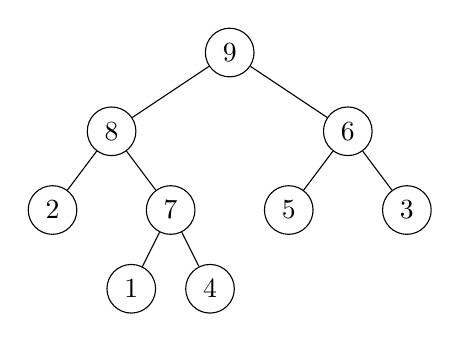
\begin{tikzpicture}[level distance=1cm,
    level 1/.style={sibling distance=3cm},
    level 2/.style={sibling distance=1.5cm},
    level 3/.style={sibling distance=1cm}
    ]
    \node[circle, draw] {9}
      child {node[circle, draw] {8}
        child {node[circle, draw] {2}}
        child {node[circle, draw] {7}
          child {node[circle, draw] {1}}
          child {node[circle, draw] {4}}
        }
      }
      child {node[circle, draw] {6}
        child {node[circle, draw] {5}}
        child {node[circle, draw] {3}}
      };
  \end{tikzpicture}
\]

\podnaloga
Razredu \verb|Drevo| dodajte metodo \verb|naloga2a(self)|,
  ki vrne \verb|True|, kadar je dano drevo sebično, in \verb|False|, kadar ni.

Časovna zahtevnost metode naj bo $O(n)$, kjer je $n$ število vrednosti v drevesu.

\podnaloga
Razredu \verb|Drevo| dodajte metodo \verb|naloga2b(self,x)|,
  ki v dano sebično drevo doda vrednost \verb|x| tako,
  da je razširjeno drevo še vedno sebično.
Pri tem lahko elemente drevesa poljubno preurejate,
  pazite le, da iz drevesa ne pobrišete nobenega elementa
  in da ne dodate nobenega drugega elementa poleg \verb|x|.

Časovna zahtevnost metode naj bo $O(\log d)$, kjer je $d$ globina drevesa.

%%%%%%%%%%%%%%%%%%%%%%%%%%%%%%%%%%%%%%%%%%%%%%%%%%%%%%%%%%%%%%%%%%%%%%
\naloga[25 točk]
V \emph{Mathematici} sestavite funkcijo \verb|naloga3[n_]|,
  ki izriše sledeče fraktale:

\begin{center}
  
\includegraphics[width=\textwidth]{gobe.pdf} \\
  \verb|naloga3[0]|\qquad\qquad\qquad
  \verb|naloga3[1]|\qquad\quad\qquad
  \verb|naloga3[2]|\qquad\qquad\qquad
  \verb|naloga3[3]|
\end{center}

%%%%%%%%%%%%%%%%%%%%%%%%%%%%%%%%%%%%%%%%%%%%%%%%%%%%%%%%%%%%%%%%%%%%%%
\naloga[25 točk]

\podnaloga
Sestavite funkcijo \verb|naloga4a[f_, sezzz_]|,
  ki na ``listih'' (vseh kosih, ki niso seznami)
  gnezdenega seznama \verb|sezzz| uporabi funkcijo \verb|f|.
Na primer:
{\small\begin{verbatim}
   In[1]:= naloga4a[f, {1, {2, 3, 4}, 5}]
   Out[1]= {f[1], {f[2], f[3], f[4]}, f[5]}
   In[2]:= naloga4a[f, {1, {2, {3, 4}, 5}, {6, 7, {}, 8}, 9}]
   Out[2]= {f[1], {f[2], {f[3], f[4]}, f[5]}, {f[6], f[7], {}, f[8]}, f[9]}
   In[3]:= naloga4a[f, {1, {2, {1, 2}, 1}, 2}]
   Out[3]= {f[1], {f[2], {f[1], f[2]}, f[1]}, f[2]}\end{verbatim}}

\podnaloga
Sestavite funkcijo \verb|naloga4b[sezzz_]|,
  ki liste gnezdenega seznama \verb|sezzz| krožno prestavi za eno mesto v levo.
{\small\begin{verbatim}
   In[1]:= naloga4b[{1, {2, 3, 4}, 5}]
   Out[1]= {2, {3, 4, 5}, 1}
   In[2]:= naloga4b[{1, {2, {3, 4}, 5}, {6, 7, {}, 8}, 9}]
   Out[2]= {2, {3, {4, 5}, 6}, {7, 8, {}, 9}, 1}
   In[3]:= naloga4b[{1, {2, {1, 2}, 1}, 2}]
   Out[3]= {2, {1, {2, 1}, 2}, 1}\end{verbatim}}

\end{document}

